\documentclass[11pt, oneside]{article} 
\usepackage{geometry}
\geometry{letterpaper} 
\usepackage{graphicx}
	
\usepackage{amssymb}
\usepackage{amsmath}
\usepackage{parskip}
\usepackage{color}
\usepackage{hyperref}

\graphicspath{{/Users/telliott_admin/Dropbox/Tex/png/}}
% \begin{center} 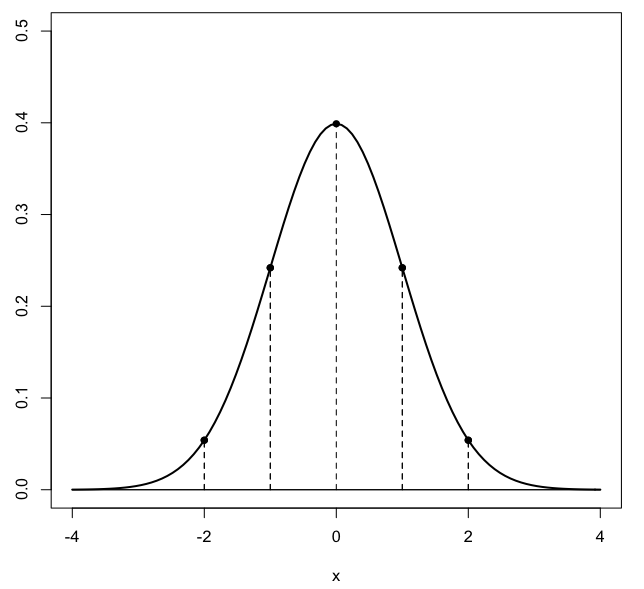
\includegraphics [scale=0.4] {gauss3.png} \end{center}

%break
\title{Polar hyperbola}
\date{}

\begin{document}
\maketitle
\Large
We can also use a focus-directrix approach to the definition of the hyperbola.  It will turn out to give the same formula as that of the ellipse and the parabola, but there are a few twists and turns along the way.

\url{http://mathworld.wolfram.com/Hyperbola.html}

\begin{center} 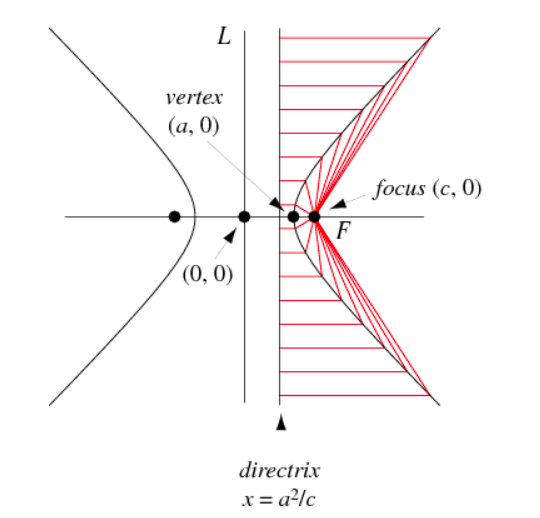
\includegraphics [scale=0.4] {hyperbola_directrix.png} \end{center}

The equation will turn out to be similar to that for the ellipse and parabola
\[ r = \frac{ep}{1 - e \cos \theta} \]
except that $e > 1$, as we will see.

First, though, recall the equation that we derived before, namely
\[ \frac{x^2}{a^2} - \frac{y^2}{b^2} = 1 \]

\subsection*{meaning of a and b}
This gives a hyperbola of the type graphed above, opening "east-west".  As we used in the derivation, $c$ is the distance from the origin to each focus.  Although the value of $x$ is never $0$, the value of $y$ can be, and at those two points we have
\[ x^2 = a^2 \]
\[ x = \pm a \]
So $a$ is the horizontal distance to points on the curve along the $x$-axis.

As for $b$, we rearrange the basic equation
\[ b^2x^2 - a^2y^2 = a^2 b^2 \]
\subsection*{asymptotes}
Associated with the hyperbola is a pair of lines called asymptotes.  Their equation is 
\[ b^2x^2 - a^2y^2 = 0 \]
Factoring
\[ (bx + ay)(bx - ay) = \]
which has solutions when
\[ y = \pm \frac{b}{a} x \]
For a hyperbola in standard orientation like this, these lines go through the origin.

\subsection*{eccentricity}
Notice that, unlike the ellipse, $a < c$.  We define the eccentricity with the same equation as for the ellipse
\[ ea = c \]
but now realize that for a hyperbola $e > 1$.

Recall that we defined
\[ b^2 = c^2 - a^2, \ \ \ \ (c > a) \]
Hence
\[ b^2 = (ea)^2 - a^2 = a^2(e^2 - 1) \]
whereas before for the ellipse we had
\[ b^2 = a^2(1 - e^2) \]

\subsection*{directrix}
For the directrix we will assume the answer, and then show that it leads to the desired properties.  From the diagram above we read that on the directrix 
\[ x = \frac{a^2}{c} \]

That is, the distance $d$ from the $y$-axis is equal to
\[ d = \frac{a^2}{c} \]

and since $c = ea$
\[ d = \frac{a}{e} \]
which is just what we had before with the ellipse:
\[ ea = c \]
\[ ed = a \]
(except that now with the hyperbola $e > 1$ and $c > a > d$ whereas before with the ellipse $e < 1$ and $d > a > c$).

On the $x$-axis the distance from the focus to the curve is $c-a$ and from the curve to the directrix is $a - d$.  We consider the ratio of the two distances
\[ \frac{c - a}{a - d} = \frac{ea - a}{a - a/e} \]
\[ = \frac{a(e -1)}{a(1 - 1/e)} \]
\[ = \frac{(e -1)}{(1 - 1/e)} \]
Multiply by $e$ on top and bottom:
\[ = e \frac{(e -1)}{(e - 1)} \]
\[ = e \]

\subsection*{definition of p}
As before, in a similar way to the directrix $d = a^2/c$, we define the focal parameter $p$ as
\[ p = \frac{b^2}{c} \]
\[ = \frac{c^2 - a^2}{c} \]
\[ = \frac{e^2a^2 - a^2}{c} \]
\[ = \frac{a^2(e^2 - 1)}{c} \]
\[ = \frac{a(e^2 - 1)}{e} \]

\subsection*{polar coordinates}
\begin{center} 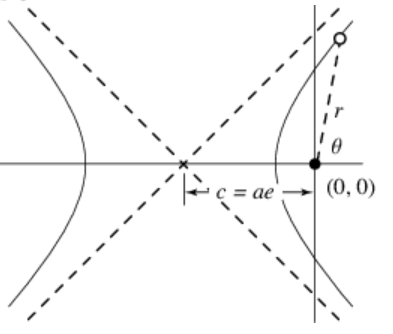
\includegraphics [scale=0.6] {hyperbola_polar.png} \end{center}
The geometric constraint is 
\[ \frac{PF}{PD} = e \]
where $PF$ is just $r$ and the problem is to evaluate the length of $PD$.
\[ PD = r \cos \theta + (c - d) \]
Hence we have that
\[ e = \frac{r}{r \cos \theta + (c - d)} \]
\[ er \cos \theta + e(c - d) = r \]
\[ r(e \cos \theta - 1) = - e(c-d) \]
\[ r = \frac{e(c - d)}{1 - e \cos \theta} \]

The numerator
\[ e(c - d) = e(ea - \frac{a}{e}) \]
\[ a(e^2 - 1) \]
\[ = ep \]
So finally we obtain:
\[ r = \frac{ep}{1 - e \cos \theta} \]
as the equation of a standard hyperbola in polar coordinates.

We recovered the same equation for all three conic sections:  parabola, ellipse and hyperbola.  The only difference is the value of $e$.  Here $e > 1$, for the parabola $e =1$ and for the ellipse $e < 1$.
\end{document}